\documentclass[11pt]{article}
\title{\textbf{Triple unit}}
\author{https://github.com/heptagons/meccano/units/triple}
\date{}

\usepackage{../../meccano}
\usepackage{tikz}
\usetikzlibrary{calc}

\begin{document}

\maketitle
\begin{abstract}
Triple unit is a group of five meccano\meccanoref strips $a,b,c,d,e$ intended to build regular polygons three consecutive perimeter sides.
This unit has three angles equal to the polygon internal angle $\theta$. 
Triple unis has been using to build the pentagon type 2 mentioned in pentagons paper\footnote{
\href{https://github.com/heptagons/meccano/blob/main/penta/pentagons.pdf}{Meccano pentagons}}.
\end{abstract}

\begin{figure}[h]
\centering
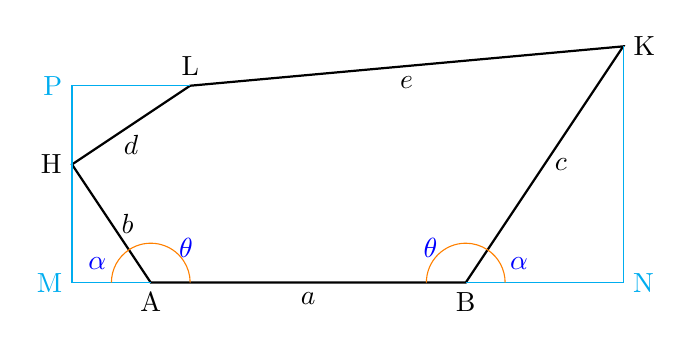
\begin{tikzpicture}
\begin{scope}[scale=0.5]
\draw[black,thick] (0,0)
-- node[below] {$a$} ++(8,0) node[below]{B}
-- node[below,right] {$c$} ++(4,6) node[right]{K}
-- node[below] {$e$} ++(-11,-1) node[above]{L}
-- node[below] {$d$} ++(-3,-2) node[left]{H}
-- node[right] {$b$} cycle node[below]{A};
\draw[cyan] (0,0)
-- ++(-2,0) node[below,left] {M}
-- ++(0,3)
-- ++(0,2) node[above,left] {P}
-- ++(3,0);
\draw[cyan] (8,0)
-- ++(4,0) node[below,right] {N}
-- ++(0,6);

\draw[orange] (0,0)+(-1,0)
 arc(180:180-atan(3/2):1) node[midway,above,left,blue] {$\alpha$}
 arc(180-atan(3/2):0:1) node[midway,above,right,blue] {$\theta$};
\draw[orange] (8,0)+(-1,0)
 arc(180:atan(3/2):1) node[midway,above,left,blue] {$\theta$}
 arc(atan(3/2):0:1) node[midway,above,right,blue] {$\alpha$};
%\draw[orange] (-2,3)+(-1.2,1.2)
 

\end{scope}
\end{tikzpicture}
\caption{Triple unit has five strips $a,b,c,d,e$}
\label{fig:triple}
\end{figure}
\end{document}